% !Mode:: "TeX:UTF-8"
\chapter{循环神经网络的轻量化压缩}
\label{cha:第三章}
% 本章节提出了一种基于动力学模型降阶方法——本征正交分解法的循环神经网络模型压缩方法。首先,介绍了循环神经网络及其变体长短期记忆网络的基本结构及其动力学模型。然后,详细介绍了本征正交分解法的原理和算法。最后,将本征正交分解法应用于循环神经网络模型压缩。实验结果表明,本征正交分解法可以有效地压缩循环神经网络模型,同时保持模型的预测性能。
时效性是RAG问答系统的关键指标之一,为提高RAG问答系统的推理效率本章节提出了一种基于动力学模型降阶方法——本征正交分解法的循环神经网络模型压缩方法。首先,介绍了循环神经网络及其变体长短期记忆网络的基本结构及其动力学模型,通过将循环神经网络表达为动力学微分方程来增加神经网络的可解释性。然后,详细介绍了本征正交分解法的原理和算法。最后,将本征正交分解法应用于循环神经网络模型压缩。实验结果表明,本征正交分解法可以有效地压缩循环神经网络模型,同时保持模型的性能。
\section{问题描述}
尽管以Transformer为核心架构的大语言模型凭借其全局注意力机制与并行化计算优势,在自然语言处理领域占据主导地位,但循环神经网络(Recurrent Neural Network, RNN)在连续提示词编码场景中仍展现出独特的应用价值与轻量化潜力\cite{liu2024gpt,liu2022p}。相较于Transformer模型依赖自注意力机制构建长程依赖所导致的高计算复杂度,RNN通过参数共享时序建模特性,能够以更低的内存开销实现连续提示词编码。这一特性使其在资源受限场景中具有显著优势。进一步地,RNN的循环结构适配轻量化压缩需求。通过动力学系统视角下的模型降阶方法,可对RNN隐藏状态进行低维投影,在保留时序动态特征的前提下实现参数的高效压缩。

% 例如,在连续提示词学习中,双向门控循环单元(BiGRU)可通过门控机制自适应调节多层级提示(如任务描述向量与检索增强上下文)的融合权重,生成上下文敏感的低维向量表示,而无需依赖Transformer的高维多头注意力计算。
伴随着神经网络的发展,出现了更多新的研究视角。有论文将神经网络看作常微分方程或动力学系统\cite{chen2018neural}。在以往的许多工作中,循环神经网络都被表示成常微分方程\cite{rubanova2019latent,mozer2017discrete},并使用动力学系统中的方法处理它。受前人工作启发,文中提出一种动力学系统模型降阶方法来降低长短期记忆网络模型隐藏层状态的维度,该方法可以压缩权重矩阵并减少计算量。

面对神经网络模型的发展,为了实现更好的性能而模型参数越来越大,于是面临着设备存储资源有限而部署困难的问题\cite{deng2020model},同时也面对边缘设备无法支持庞大的计算量所需要的能源问题\cite{han2015deep}。需要能够同时压缩模型参数和推理计算量的模型压缩方法来解决神经网络的工程实践问题。循环神经网络与卷积神经网络不同,循环神经网络的前向传播通常由时间序列决定并且每一时间步上的隐藏层状态使用相同的权重矩阵。隐藏层状态包含着大量的特征信息,其节点数量决定了循环神经网络的权重矩阵和计算量的大小。隐藏层状态的维度是一种超参数,往往无法定义最合适的维度,在大多数情况下,设置的隐藏层维度会高于实际编码特征所需要的维度,这就造成了参数的冗余。所以希望提出一种方法能够将隐藏层的维度压缩至合适的大小,则可以减少参数量和计算量。因此,提出了一种基于本征正交分解的模型压缩方法,该方法的原理是用低维向量近似原始的高维向量。
实验应用了一个两层长短期记忆网络去完成在固定时间序列的分类问题,并使用本征正交分解的方法可以在精度损失很少的情况下,将其压缩。

% 在自然语言处理领域,Transformer大语言模型凭借全局注意力机制与并行化计算优势占据主导地位,但循环神经网络(RNN)在连续提示词编码场景中仍具独特价值与轻量化潜力\cite{liuGPTUnderstandsToo2023,liuPTuningV2Prompt2022}。与Transformer依赖自注意力机制构建长程依赖导致高计算复杂度不同,RNN通过参数共享时序建模,能以更低内存开销实现连续提示词编码,使其在资源受限场景(如边缘计算设备或实时交互系统)中更具优势。例如,双向门控循环单元(BiGRU)可通过门控机制自适应调节多层级提示的融合权重,生成上下文敏感的低维向量表示,无需依赖Transformer的高维多头注意力计算。此外,RNN的循环结构天然适配轻量化压缩需求,通过动力学系统视角下的模型降阶方法(如本征正交分解),可对RNN隐藏状态进行低维投影,在保留时序动态特征的前提下实现参数的高效压缩。

% 随着神经网络的发展,出现了多种研究视角,有论文将其视为常微分方程或动力学系统\cite{chenNeuralOrdinaryDifferential2019},许多工作中循环神经网络被表示为常微分方程\cite{rubanovaLatentODEsIrregularlySampled,mozerDiscreteEventContinuous2017}并使用动力学系统方法处理。受此启发,本文提出一种动力学系统模型降阶方法来降低长短期记忆网络模型隐藏层状态的维度,以压缩权重矩阵并减少计算量。然而,神经网络模型为追求更好性能导致参数规模越来越大,面临设备存储资源有限、部署困难的问题\cite{dengModelCompressionHardware2020},同时边缘设备也难以支持庞大计算量所需的能源\cite{hanDeepCompressionCompressing2016},因此需要能同时压缩模型参数和推理计算量的模型压缩方法来解决工程实践问题。

% 循环神经网络与卷积神经网络不同,其前向传播由时间序列决定,且每一时间步上的隐藏层状态使用相同的权重矩阵。隐藏层状态包含大量特征信息,其节点数量决定了循环神经网络的权重矩阵和计算量的大小。隐藏层状态的维度是一种超参数,往往难以定义最合适的维度,大多数情况下设置的隐藏层维度会高于实际编码特征所需要的维度,造成参数冗余。因此,本文提出一种基于本征正交分解的模型压缩方法,其原理是用低维向量近似原始的高维向量。实验中,应用了一个两层长短期记忆网络完成固定时间序列的分类任务,并使用本征正交分解的方法,在几乎不损失精度的情况下成功将其压缩。

\section{本征正交分解法}
本征正交分解法\cite{nomura1993structure}作为一种基于数据驱动的降维方法,其核心思想是通过提取高维动力学系统状态空间中的主导信息,构建低维子空间以近似原始系统的方法。该方法能够通过一组正交基降低非线性动力学系统模型的维度,是一种常见的模型降阶方法,其在流体力学、结构动力学等领域已得到广泛应用。在文中被引入神经网络模型压缩领域,为解决循环神经网络(RNN)参数量冗余与计算效率问题提供了新思路。
本征正交分解法(POD)的核心思想是将$k$个样本点的$n$维数据,投影到$m$维,即$n$维的数据可以被$m$维的数据近似,并且$m<<n$。假设有$k$个采样数据${x_1},{x_2},...,{x_k}$其中 ${x_i}\in {R} ^{n}$记作
\begin{equation}
  \label{eq:1}
X = [ {x_1},{x_2},...,{x_k}]  \in {R} ^{n \times k}
\end{equation}
通过奇异值分解法(Singular Value Decomposition, SVD)计算样本数据 的一组正交基向量$\{ {\phi _i}\} _{i = 1}^n$,使对于每一个${x_i} \in {R}^n,i \in [1,k]$都能够被表示为正交基向量的线性组合
\begin{equation}
  \label{eq:2}
{x_i} = {y_{1i}}{\phi _1} + {y_{2i}}{\phi _2} +  \cdots  + {y_{ni}}{\phi _n},{\rm{ }}{y_{ji}} \in {R}
\end{equation}
由于在SVD计算过程中基向量$\{ {\phi _i}\} _{i = 1}^n$按照能代表的信息量递减排序,所以可以用信息密度最高的前$m$项来近似原始样本数据,即
\begin{equation}
  \label{eq:3}
  {x_{i(m)}} = {y_{1i}}{\phi _1} + {y_{2i}}{\phi _2} +  \cdots  + {y_{mi}}{\phi _m},{\rm{ }}{y_{ji}} \in {R}
\end{equation}
% 记作${x_m} = \phi {{\bf{y}}_m},{{\bf{y}}_m} \in \mathbf{R}^m$。
将原始数据和近似数据之间的误差定义为
\begin{equation}
  \label{eq:4}
{\varepsilon ^2} = \sum\limits_{i = 1}^m {\left\| {{x_i} - {x_{i(m)}}} \right\|_2^2}  = \sum\limits_{j = m + 1}^n {\phi _j^T} X{X^T}{\phi _j}
\end{equation}
其中$X = [ {x_1},{x_2},...,{x_k}] $。通过构建拉格朗日方程最小化误差,得到最小误差下的一组正交基向量$\{ {\phi _i}\} _{i = 1}^n$为采样数据点${X^T}$的右奇异值矩阵$V$ \cite{chatterjee2000introduction}。数据点可通过奇异值分解表示为
\begin{equation}
\label{eq:5}
  {X^T} = U\Sigma  {V^T}
\end{equation}
其中$X$为采样数据点$\{ {x_1},{x_2},...,{x_k}\}  \in {{R}^{n \times k}}$,$\Sigma $为降序排列的奇异值对角矩阵,$U$是左奇异值矩阵,$V$是右奇异值矩阵。
% 并且满足
% \begin{equation}
% \label{eq:6}
% UV = I
% \end{equation}
% 其中$I$为单位矩阵。
下面介绍POD的基本降阶过程。
对于以下非线性离散动力学系统
\begin{equation}
\label{eq:7}
\left\{ \begin{array}{l}
  {x_{t + 1}} = f({x_t},{u_t})\\
  {y_t} = g({x_t},{u_t})
  \end{array} \right.
\end{equation}
其中函数$f( \cdot ) \in {{R}^n}$和函数$g( \cdot ) \in {{R}^o}$为非线性函数,${u_t} \in {{R}^i}$为系统输入,${y_t} \in {{R}^o}$为系统输出。取一定连续时间内的系统状态
\begin{equation}
\label{eq:8}
X = [{x_1},{x_2},...,{x_k}]  \in {R}^{n \times k}
\end{equation}
为需要降阶近似的数据。设矩阵$V,W \in {{R}^{n \times m}}$$(m<n)$满足
\begin{equation}
\label{eq:9}
{W^T}V = {I_m}  
\end{equation}
其中$I_m$为单位矩阵。
根据上文方法得到$m$维基向量矩阵
\begin{equation}
\label{eq:10}
{\varPhi  _m} = [{\phi _1},{\phi _2},...,{\phi _m}]
\end{equation}
令
\begin{equation}
\label{eq:11}
V = W = {\varPhi  _m} \in {{{R}}^{n \times m}}
\end{equation}
则${\hat x_t} = \varPhi  _m^T{x_t}$为${x_t}$到$\varPhi  _m^T$所在空间上的投影。$W$由采样数据 的右奇异值矩阵前$m$项组成。系统\ref{eq:7}降阶后的系统为
\begin{equation}
\label{eq:12} 
\left\{ \begin{array}{l}
  {x_{t + 1}} = {W^T}f(V{{\hat x}_t},{u_t})\\
  {y_t} = g(V{{\hat x}_t},{u_t})
  \end{array} \right.
\end{equation}
其中${\hat x_t} \in {{R}^m}$。可以通过投影矩阵$W$, $V$得到降阶系统。
\section{动态循环神经网络}
循环神经网络作为时间序列建模常用模型,在不同采样时间下具有连续变化的状态,每个采样时间下的结果取决于上一个采样的结果和当前的输出,并且每次计算的系数矩阵和函数相同,这点与动力学系统类似,且由于激活函数的存在,可以将循环神经网络视作非线性动力学系统。为验证循环神经网络与动力学系统的相似性,分别使用循环神经网络和动力学系统模型简单对一个时间序列进行建模,并比较结果。
实验使用RNN模型拟合一个正弦函数映射到余弦函数的序列模型。自定义一个32节点单层循环神经网络,使用正弦函数作为输入,余弦函数作为标签训练输出,采样频率为1/0.0625π HZ。将得到训练后的RNN模型参数作为动力学系统的微分方程形式,将RNN网络表示为
\begin{equation}
\label{eq:13}
{h_{t + 1}} = f({h_t} + {x_t})
\end{equation}
其中$h_t$代表$t$时刻隐藏层状态,$x_t$代表$t$时刻输入,$f$为RNN结构,由RNN训练后的模型参数决定。将公式\ref{eq:13}等式两边同时减去$h_t$得到
\begin{equation}
\label{eq:14}
{h_{t + 1}} - {h_t} = f({h_t} + {x_t}) - {h_t}
\end{equation}
将公式\ref{eq:14}连续化为微分方程形式得到
\begin{equation}
\label{eq:15}
  {\dot h_t} = \frac{1}{{\Delta t}}(f({h_t} + {x_t}) - {h_t})
\end{equation}
通过这种变换得到了 的微分方程,使用积分器得到后续状态,即ODE-RNN的前向传播,根据数据得到图像, 实验结果如图\ref{fig:函数拟合结果}所示。
\begin{figure}[!htbp]
  \centering
  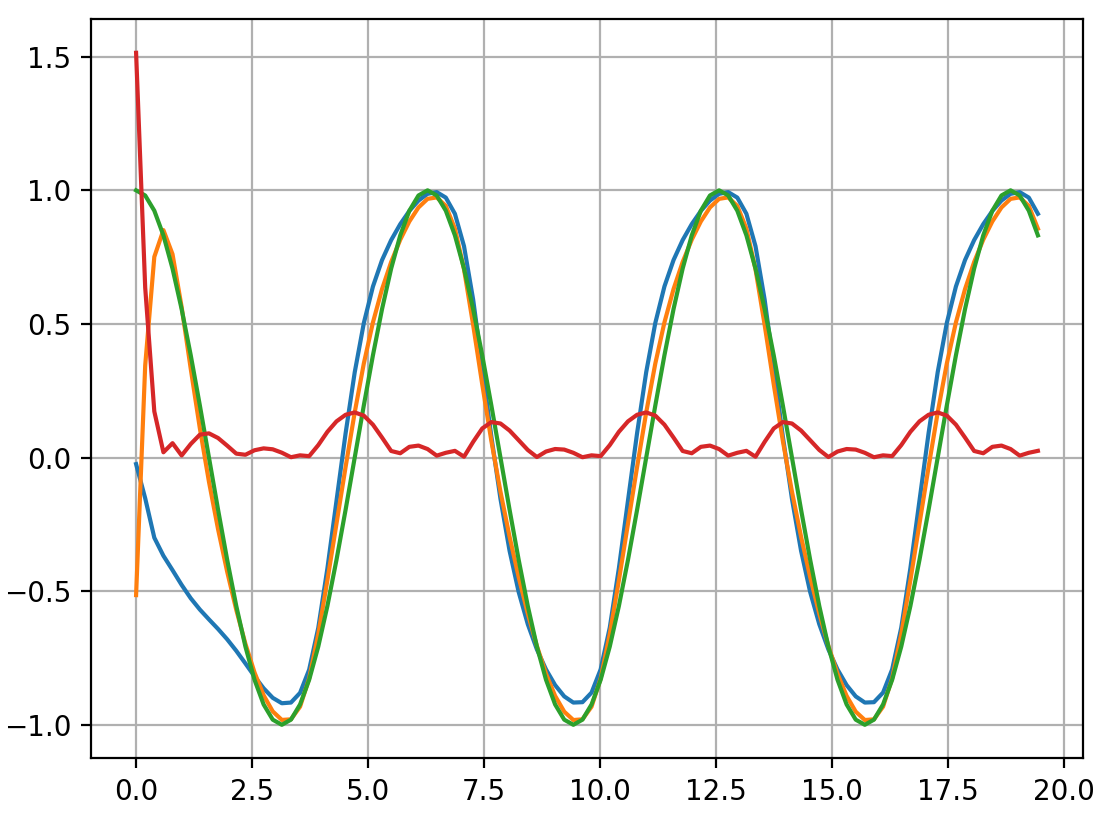
\includegraphics[width=0.7\textwidth]{函数拟合结果.png}
  \bicaption{函数拟合结果}{Comparison of Cosine Function Modeling}
  \label{fig:函数拟合结果}
\end{figure}
绿色波形为标准余弦信号,橙色波形为动力学系统建模,红色波形为二者之间的差,蓝色波形为使用POD方法降阶后的结果。实验结果表明将原本训练好的RNN参数带入到微分方程中能够完成功能,表明了在参数相同时动力学系统与神经网络的一致性。
尽管传统循环神经网络在时间序列建模中可通过离散化常微分方程形式表征
其动力学特性,但其在长期依赖任务(如长程时间序列分类)中表现受限。这一局限性主要源于梯度消失/爆炸等问题,导致网络难以有效捕捉跨时间步的时序关联性。
为解决此问题,长短期记忆网络(Long Short-Term Memory, LSTM)\cite{hochreiter1997long}通过引入门控机制(输入门、遗忘门、输出门)重构了隐藏状态的动态演化过程。具体而言,遗忘门通过可学习的权重系数调节历史信息的保留比例,而输入门则动态控制当前输入的融合强度,从而实现对长期依赖的显式建模。实验表明,门控机制对复杂时序模式捕获的有效性。
然而,LSTM的高参数维度(如隐藏层维度为128时参数量达70k)导致其在资源受限场景下的部署面临挑战。为此,本征正交分解(Proper Orthogonal Decomposition, POD)方法被引入模型压缩领域。通过提取LSTM隐藏状态空间中的主导信息,POD将原始高维状态投影至低维子空间,并重构动力学方程。这一方法通过保留关键信息,在轻量化与性能间实现了高效平衡。

对于一个多层长短期记忆网络(如图\ref{fig:LSTM}所示),
\begin{figure}[hbp]
  \centering
  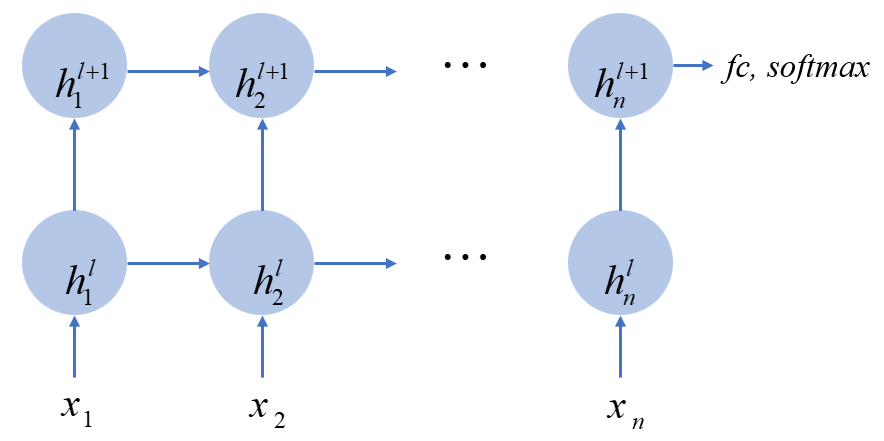
\includegraphics[width=0.7\textwidth]{多层长短期记忆网络结构.png}
  \bicaption{多层长短期记忆网络结构}{ the Multilayer LSTM Structure}
  \label{fig:LSTM}
\end{figure}
可以被表示为以下非线性的离散动力学系统
\begin{equation}
\label{eq:16}
h_{t + 1}^l = f(W_i^l{x_{t + 1}} + W_h^lh_t^l + {b^l})
\end{equation}
\begin{equation}
\label{eq:17}
h_{t + 1}^{l + 1} = f(W_i^{l + 1}h_{t + 1}^l + W_h^{l + 1}h_t^{l + 1} + {b^{l + 1}})
\end{equation}
其中$f( \cdot )$为长短期记忆单元,$W_i^l \in {R^{n \times i}}$为第$l$层的输入矩阵,$W_h^l \in {R^{n \times n}}$是第$l$层的隐藏层矩阵,${b^l} \in {R^n}$为第$l$层的偏置。通过本征正交分解法计算投影矩阵$V \in {R^{n \times m}}$($m$是隐藏层 的新维度),并用其线性组合$h = V\hat h$来近似$h$。$\hat h \in {R^m}$为新隐藏层的系数矩阵,用$V\hat h$替换等式\ref{eq:16}和等式\ref{eq:17}中的$h$,得到
\begin{equation}
  \label{eq:18}
  \hat h_{t + 1}^l = {U^l}f(W_i^l{x_{t + 1}} + W_h^l{V^l}\hat h_t^l + {b^l})
  \end{equation}
\begin{equation}
  \label{eq:19}
  \hat h_{t + 1}^{l + 1} = {U^{l + 1}}f(W_i^{l + 1}{V^l}\hat h_{t + 1}^l + W_h^{l + 1}{V^{l + 1}}\hat h_t^{l + 1} + {b^{l + 1}})
  \end{equation}
其中$U^l$为$V^l$的转置,满足$U=V^T$。新的模型可以被表示为
\begin{equation}
  \label{eq:20}
  \hat h_{t + 1}^l = {U^l}f(W_i^l{x_{t + 1}} + \hat W_{\hat h}^l\hat h_t^l + {b^l})
  \end{equation}
\begin{equation}
  \label{eq:21}
  \hat h_{t + 1}^{l + 1} = {U^{l + 1}}f(\hat W_i^{l + 1}\hat h_{t + 1}^l + \hat W_{\hat h}^{l + 1}\hat h_t^{l + 1} + {b^{l + 1}})
  \end{equation}
其中$\hat W_{\hat h}^l = W_h^l{V^l} \in {R^{n \times m}}$,$\hat W_i^{l + 1} = W_i^{l + 1}{V^l} \in {R^{n \times m}}$,$\hat W_{\hat h}^{l + 1} = W_h^{l + 1}{V^{l + 1}} \in {R^{n \times m}}$, $\hat h \in {R^m}$ 。

通过将隐藏状态投影到较低的状态,可以获得具有较少参数和隐藏状态的模型,如图\ref{fig:原始模型和压缩模型的结构}所示,直观地展示新模型与原始模型在参数和隐藏层维度上的维度差异。其中$i$,$f$,$c$,$o$分别代表输入门、遗忘门、控制们和输出门。$W$,$V^T$分别代表每个们的权重矩阵和投影矩阵,$b$代表偏执,$h_t$,$c_t$,$o_t$分别代表$t$时刻的隐藏层状态、控制状态和输出状态。符号$\hat  \cdot $标志压缩后的模型参数。

在长短期记忆网络模型中,每层网络的隐藏层都有四个门控系数矩阵和输入系数矩阵。
降低以上矩阵的维度来达到压缩的目的。本小节通过将循环神经网络以动力学系统的方式表达,增加了神经网络的可解释性。

\begin{figure}[!htbp]
  \centering
  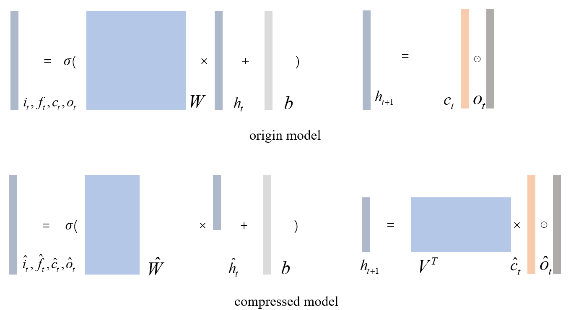
\includegraphics[width=0.74\textwidth]{原始模型和压缩模型的结构.png}
  \bicaption{原始模型和压缩模型的结构}{The Structure of the Original Model and Compressed Model.}
  \label{fig:原始模型和压缩模型的结构}
\end{figure}
\section{实验设置}
实验使用一个两层,隐藏层维度为72的长短期记忆网络来验证该方法的有效性。
实验使用UCI-HAR数据集\cite{anguita2012human}验证方法效果。UCI-HAR数据集是一个广泛应用于人类活动识别领域的公开数据集,它通过在智能手机上搭载的传感器收集了30名志愿者在进行六种日常活动(步行、上楼梯、下楼梯、静坐、站立和平躺)时产生的动态数据。这些数据由加速度计和陀螺仪以50Hz的频率采集得到,涵盖了三轴的线性加速度和角速度信息。在数据预处理阶段,研究者们通过噪声滤波器和巴特沃斯低通滤波器对原始数据进行了清洗和分离,以区分重力和身体运动分量,并计算了包括时域和频域在内的561个特征向量。数据集被分为训练集和测试集,其中训练集包含了21名志愿者的数据,而测试集则包含了剩余9名志愿者的数据。数据集有6个分类结果,9个特征和128次时间序列采样。综上,确定模型的输入系数矩阵、输出系数矩阵和时间长度,一共包含60k参数。
首先在Pytorch框架下利用标准LSTMcell和Adam优化器训练原始大小的模型。得到在测试集上准确度为85\%的基线模型。再利用本征正交分解压缩的模型与之进行对比。
将网络看作一个关于输入为$x$,输出为$y$,隐藏层为$h$,全连接层作为输出函数的非线性系统
\begin{equation}
  \label{eq:22}
\left\{ \begin{array}{l}
  {h_{t + 1}} = f({h_t},{h_t})\\
  {y_t} = fc({h_t})
  \end{array} \right.
\end{equation}
其中$fc( \cdot )$为全连接层。模型的隐藏层$h_i^l$可以被看作是非线性系统的状态变量,记作$\{ h_1^l,h_2^l,...,h_n^l\}$。模型的每一层隐藏层都分别用一组正交基$V$表示。正交基$V$可由算法\ref{algo:projecting_matrix}计算。
\begin{algorithm}[!htbp]
  \caption{得到投影矩阵}
  \label{algo:projecting_matrix}
  \DontPrintSemicolon
  \SetKwInOut{Input}{输入}
  \SetKwInOut{Output}{输出}
  \SetKwFunction{LSTM}{LSTM}
  \SetKwFunction{Average}{average}
  \SetKwFunction{SVD}{svd}
  
  \Input{1 批次训练数据,长短期记忆网络模型}
  \Output{投影矩阵 $V$}
  
  \vspace{5pt}
  
  $\{h_1, h_2, ..., h_n\} = \LSTM(\text{dataset})$\;
  $\mathbf{H} = \Average(\sum_{i=1}^{\text{batch\_size}} \{h_1, h_2, ..., h_n\})$\;
  $U \Sigma V' = \SVD(\mathbf{H}')$\;
  $V = V[:, 1:m]$\;
  
\end{algorithm}

在本研究中,为提升矩阵$V$的泛化性能,引入平均值函数 $average(\cdot)$,通过对所有输入数据进行平均值计算,降低模型的过拟合风险,增强其对未知数据的泛化能力。奇异值分解(SVD)函数$svd(\cdot)$被应用于计算矩阵$V$,通过分解矩阵揭示其内在特征,降低维度,去除冗余信息,提高模型的计算效率和泛化能力。投影矩阵$V$可以从模型的任意状态序列中导出,为模型架构提供高度灵活性,但不同的$V$矩阵选择可能导致不同程度的精度损失,需权衡泛化能力和精度。计算平均值的方法在数据量较大的情况下,能够更有效地整合信息,提升模型的泛化能力,通过在更大的数据集 的隐藏层状态$h$上计算平均值,捕捉数据分布特征,减少估计偏差。尽管利用复数数据在优化矩阵$V$方面取得了显著成效,但理论上还存在其他潜在的方法,如正则化技术或深度学习方法,可能进一步提升矩阵$V$的性能。
\section{结果分析}
原始自定义长短期记忆网络作为基线模型,利用基于本征正交分解的模型压缩方法将模型压缩至不同压缩比,利用不同隐藏层节点数量区分压缩模型,验来证模型性能和方法的科学性。
\begin{table}[htb]
  \centering
  \begin{minipage}[t]{0.8\linewidth}
    \bicaption[不同压缩维度下结果]{不同压缩维度下结果}[The Result in Different Compression Dimensions]{The Result in Different Compression Dimensions}
    \label{tab:compression-results}
    \begin{tabularx}{\linewidth}{lXXXX}
      \toprule[1.5pt]
      {\heiti 模型} & {\heiti 参数压缩比} & {\heiti 参数量} & {\heiti 计算量压缩比}  & {\heiti 准确率} \\\midrule[1pt]
      基线 & - & 9.5M & - &  85.0\% \\
      HNN=72 & - & - & - &  85.0\% \\
      HNN=64 & 93.5\% & 7.5M & 79.2\% &  84.6\% \\
      HNN=54 & 73.7\% & 5.4M & 56.7\% &  81.8\% \\
      HNN=46 & 52.6\% & 3.9M & 41.3\% &  81.8\% \\
      HNN=36 & 34.4\% & 2.4M & 25.6\% &  80.0\% \\
      HNN=28 & 22.7\% & 1.5M & 15.7\% &  66.1\% \\
      HNN=18 & 11.3\% & 0.6M & 6.7\% &  64.6\% \\
      \bottomrule[1.5pt]
    \end{tabularx}
  \end{minipage}
\end{table}
该方法的本质是通过对模型的降维,提取主要成分,压缩参数信息来实现模型的压缩。理论上,使用该方法处理模型时,模型性能会随着维度的减少而下降,所以当维度不变时,等价于对模型参数进行线性变化,模型性能不会有改变,如表\ref{tab:compression-results}所示。当隐藏层维度维持在72时,没有将高维数据向低维数据投影,无信息压缩,只进行了线性变换,故无精度损失,符合POD方法的理论基础。当隐藏层维度压缩至64时,精度只损失0.4\%,说明从72维压缩至64维所减少的维度均为冗余信息,本身不代表数据特征。压缩至36维时精度均无明显损失,当维度继续减少至36以下时,精度出现了大幅度下降,说明极低维空间(如HNN=28)无法表征复杂时序模式,导致关键模态丢失。证明主要关键信息在36维,此时已将模型压缩至34.4\%,已经减少了大量的冗余参数,并且能够基本确定该数据和模型下的最佳隐藏层维数范围。

由于POD方法为数据驱动方法,关键降阶投影矩阵$V$是由样本数据计算得到,单独每个样本都可以计算出一组投影矩阵$V$,实验对比了优化方法和随机选取一组数据计算的投影矩阵,实验结果如表\ref{tab:model-accuracy-comparison}、图\ref{fig:优化前后模型准确率对比}所示。

\begin{table}[htb]
  \centering
  \begin{minipage}[t]{0.8\linewidth}
    \bicaption[优化前后模型准确率对比]{优化前后模型准确率对比}[Comparison of Model Accuracy Before and After Optimization]{Comparison of Model Accuracy Before and After Optimization}
    \label{tab:model-accuracy-comparison}
    \begin{tabularx}{\linewidth}{lXXXX}
      \toprule[1.5pt]
      {\heiti 模型} & {\heiti 参数压缩比} & {\heiti 优化前准确率} & {\heiti 优化后准确率} \\\midrule[1pt]
      基线 & - & 85.0\% & 85.0\% \\
      HNN=72 & - & 85.0\% & 85.0\% \\
      HNN=64 & 93.5\% & - & 84.6\% \\
      HNN=54 & 73.7\% & 76.6\% & 81.8\% \\
      HNN=46 & 52.6\% & 75.1\% & 81.8\% \\
      HNN=36 & 34.4\% & 78.1\% & 80.0\% \\
      HNN=28 & 22.7\% & 55.5\% & 66.1\% \\
      HNN=18 & 11.3\% & 18.3\% & 64.6\% \\
      \bottomrule[1.5pt]
    \end{tabularx}
  \end{minipage}
\end{table}

\begin{figure}[!htbp]
  \centering
  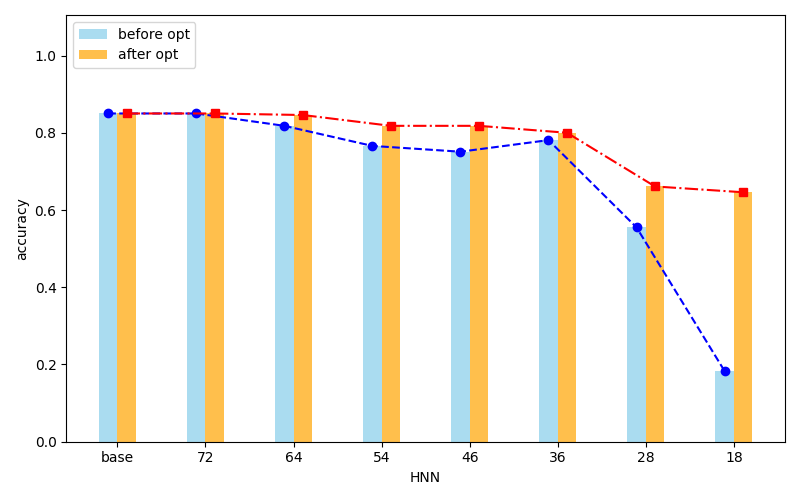
\includegraphics[width=0.8\textwidth]{优化对比.png}
  \bicaption[优化前后模型性能对比]{优化前后模型性能对比}{Comparison of Model Performance Before and After Optimization}
  \label{fig:优化前后模型准确率对比}
\end{figure}
图\ref{fig:优化前后模型准确率对比}实验结果表明,基于大规模训练数据构建的投影矩阵$V$可显著提升本征正交分解(POD)的模型压缩效果,其优化效果与降维程度呈正相关。当隐藏层维度压缩至36以下时(对应压缩比大于65\%),优化后模型的分类准确率较未优化基线平均提升1.9\%,验证了高维状态空间中关键维度的统计特性对压缩性能的关键影响。进一步分析显示,单一训练样本构建的投影矩阵因覆盖状态空间有限,易受局部动态特征干扰,导致压缩模型泛化能力下降,而基于多批次数据联合优化的投影矩阵,能够有效提取共性特征,特别在当维度降低至36以下,数据已丢失关键信息维度时,能够显著提高压缩后的模型性能。这一现象表明,投影矩阵的泛化性能本质上取决于训练数据分布的覆盖范围,当样本量不足时,POD易陷入局部最优解,而大规模数据驱动的策略可缓解非线性特征丢失的问题。

为证明POD算法的优越性,对比了现有对RNN类网络的压缩方式,与SVD\cite{xue2013restructuring}方法进行对比,实验结果如表\ref{tab:method-comparison}所示。
\begin{table}[htb]
  \centering
  \begin{minipage}[t]{0.8\linewidth}
    \bicaption[方法对比结果]{方法对比结果}[Comparison results]{Comparison Results}
    \label{tab:method-comparison}
    \begin{tabularx}{\linewidth}{lXXX}
      \toprule[1.5pt]
      {模型} & {准确率(SVD)} & {准确率(POD)} & {压缩比(POD)} \\\midrule[1pt]
      基线 & 85.0\% & 85.0\% & - \\
      HNN=72 & 85.0\% & 85.0\% & - \\
      HNN=64 & 62.9\% & 84.6\% & 93.5\% \\
      HNN=54 & 61.8\% & 81.8\% & 73.7\% \\
      HNN=46 & 33.7\% & 81.8\% & 52.3\% \\
      HNN=36 & 35.5\% & 80.0\% & 34.4\% \\
      \bottomrule[1.5pt]
    \end{tabularx}
  \end{minipage}
\end{table}

首先在模型的准确率上,POD方法和SVD方法在没有后续微调的静态对比实验中,性能明显优于SVD方法;其次在压缩效率上,SVD方法通过将系数矩阵低秩分解为两个矩阵并利用参数共享来减少参数,这种方法在压缩至同样的隐藏层节点上,压缩效率远远不及POD方法,并且只有在隐藏层节点数小于原始节点数量的一半时才有明显压缩效果,并且SVD方法通过两个低秩矩阵近相乘似一个系数矩阵时,会额外增加模型的计算量,而POD方法在保证压缩效率的同时也显著降低了模型推理时的计算量。因此,POD方法在模型精度、压缩效率和计算量三个层面均优于SVD方法。由于POD方法只在模型内部降低维度,输出维度与原始模型不变,所以当模型应用于文本嵌入等任务时,可以在不降低文本嵌入维度的前提下进行模型的压缩和加速。对于多模型合作任务下,能够保持输入输出向量为度不变,在压缩后不需要改变前后模型的输入输出维度,节省了计算资源,提高了计算效率。
\section{本章小结}
为提高RAG问答系统的时效性,本文提出了一种新的模型压缩方法,基于模型降阶方法——本征正交分解法来压缩循环神经网络。该方法可使原始模型具有最优的隐藏节点数,用较小的模型尺寸实现较高的准确率。实验中原始模型很小,总参数只有60k,因此可以将其视为紧凑模型。紧凑模型比参数规模较大的稀疏模型更难在不损失精度的情况下进行压缩。如果紧凑模型的精度损失可以控制在5\%以内,稀疏模型也可以用同样的方式在精度损失更小的情况下压缩模型参数。提出的方法可以应用于长短期记忆网络等具备时间序列特征的神经网络的压缩任务。这种新方法可以将模型大小减少到三分之一,将计算量减少到四分之一,并在精度上将损失控制在5\%。这同时也是一种不经过微调的直接调整网络结构的方法,因此它也可以与权重量化等压缩方法相结合,构建一个紧凑高效的模型。通过动力学系统的模型降阶方法来分析神经网络模型并对其压缩,将循环神经网络用动力学系统微分方程\ref{eq:15}的形式表达,用微分方程和积分的形式替代原始的隐藏层循环计算增加了对神经网络模型的解读视角和可解释性。

本章内容已发表会议论文并EI检索。
